\chapter{数学导论 - 概率统计基础:随机变量}
\begin{figure}[ht]
  \centering
  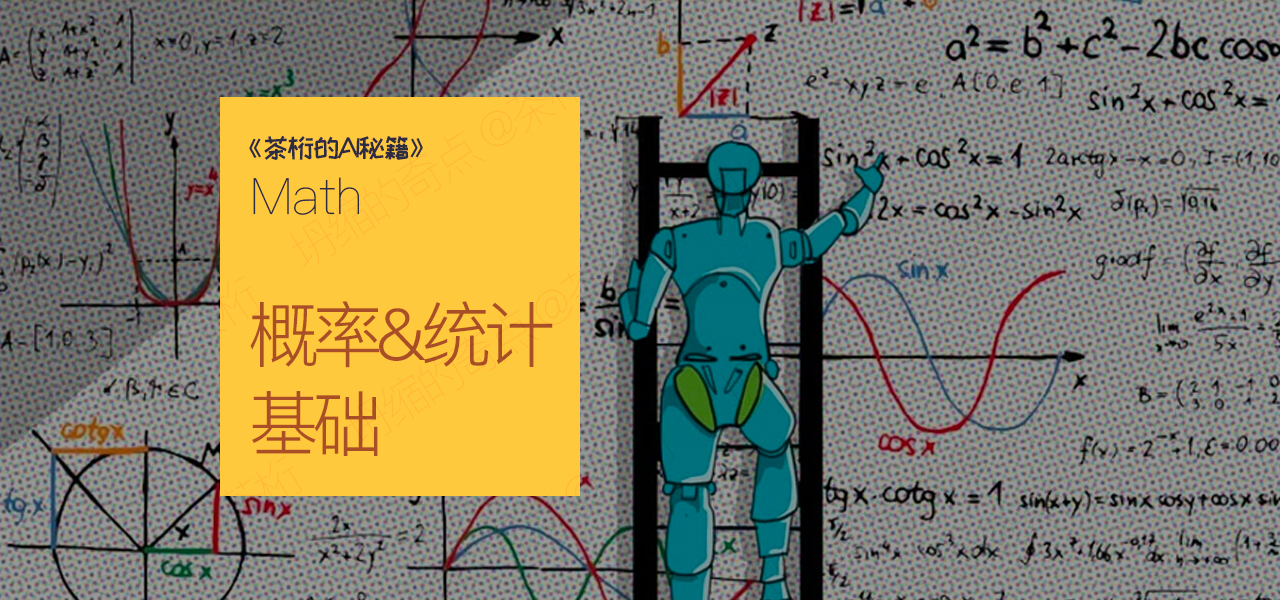
\includegraphics[width=1\textwidth]{asset/96cee23e-7016-44d9-909d-28b64c0b98e7.png}
\end{figure}
\newpage

本节课, 开始学习概率\&统计. 

我的课程的内容其实是比较核心的内容了, 也就是不需要大家特地去拾起什么高等代数这些书. 那些不需要, 也比较耽误时间. 

\section{概率\&统计}

正式开始之前, 先来看一下这几个描述:

\begin{enumerate}
  \item 平时不好好学习,考试的时候\textcolor{blue}{不确定}能否及格
  \item 太阳\textcolor{blue}{一定}是从东方升起的
  \item 绝对\textcolor{blue}{不可能}先经历明天, 再经历昨天
  \item 赌徒\textcolor{blue}{有可能}在赌场用100美元赢到1,000万美元
\end{enumerate}

这四句话里面都有一些「表示程度」的词语, 我不知道大家有没有注意到, 比如说「不确定」、「一定」、「不可能」、「有可能」, 这些就代表了在概率里面要讨论的三种事件. 

首先说到不可能, 对应着\textbf{不可能事件}; 而一定怎么样怎么样, 就对应\textbf{必然事件}; 

不可能事件就是一定不可能发生的; 必然事件是一定发生; 

剩下的不确定或者说有可能, 对应的\textbf{随机事件}, 就是它既有可能发生, 也有可能不发生. 这一部分, 就是概率学里面关注的一个重点. 因为前两种情况都都太简单了, 没研究的必要. 

概率有一个取值范围, 取值范围为0到1之间. 可以把它理解成一个百分比, 1就是100\%. 不可能比100\%还多了, 不会像361度那样, 多一度的热爱. 科学不讲这个东西, 100\%就是满了, 0就是0\%. 所以概率取值范围是在0-1之间. 

100\%发生的事件不就是一定发生的吗? 所以$P=1$对应必然事件. 0\%的可能性发生的事件就是一点可能都没有, 所以它是不可能实现. 介于两者之间就是随机的, 就是概率发生的大小. 30\%、50\%、70\%都是不确定的. 

\begin{itemize}
  \item 概率的取值范围: $0 \leq P \leq 1 $
  \item $P = 0$: 不可能事件 
  \item $P = 1$: 必然事件 
  \item \textcolor{red}{$0 < P < 1$: 随机事件 <== 概率学关注的重点}
\end{itemize}

来看一个抛硬币的例子: 抛硬币会有两种结果, 要么正面要么反面. 

\begin{figure}[ht]
  \centering
  
\includegraphics[width=0.7\textwidth]{asset/28420cc4-afeb-4064-97ec-359a2ff38dee.png}
  \caption{抛硬币}
  \label{fig:img5_1}
\end{figure}

当然我相信这个时候肯定有些同学心里面会潜意识的来一句抬杠: “它有可能抛之后还立起来呢”. 确实, 之前也看到过一篇报道就是说有一个大学教授带着他几个学生做抛硬币的实验, 还真抛出来一次立起来. 然后他们通过一系列“严谨的计算”\footnote{这个严谨打个双引号, 因为别的人也看不懂}, 立起来发生的概率是几亿分之一, 所以这个就不好说了. 

概率学上面说的抛硬币是一种抽象化的模型, 就是不扯那些其他乱七八糟东西, 什么立起来, 就把它想象成一个理想化的模型, 要么正面要么反面. 它们出现正面或者反面的概率是相等的, 都是1/2. 

每一次抛硬币就是一次随机事件, 这个事件有可能是正面朝上, 也有可能是反面朝上, 事先不能够确定. 然后根据抛硬币的模型可以提出三个问题:

\begin{itemize}
  \item 第一个问题: 单次抛掷, 正面朝上反面朝上的概率都是1/2, 那么第一次和第二次都出现正面朝上的概率应该怎么样计算? 
  \item 第二个问题: 甲是一个普通人, 他抛硬币正面朝上概率如前所述就是正面朝上0.5, 反面朝上也0.5. 乙是一个赌神, 他有一些办法,可以使正面朝上的概率是0.7. 那怎么描述让乙来抛硬币时正面朝上的概率? 直接说P等于0.7吗? 但是在普通人抛硬币的情况下, 这个P正面朝上是等于0.5. 同一个东西就出现不同的结果了. 
  \item 第三个问题: 第一次第二次抛掷均是正面朝上, 那第三次抛掷还出现正面朝上的概率还是1/2吗? 会不会和前两次有关呢? 
\end{itemize}

\section{联合概率}

先来看一下第一个问题, 第一个问题是说, 单次抛掷正面朝上反面朝上都是1/2. 那两次都正面朝上概率怎么样计算? 

首先, 这个事件是由两个先后的步骤组成: 第一次和第二次. 然后这个事件的概率是有两个步骤各自的概率相乘得到的. 第一次正面朝上在这里用 $P_{\mbox{正正}}$ 来表示, 两次都是正, 等于$\frac{1}{2} \times \frac{1}{2}$, 所以两次都出现正面的概率是1/4: 

\begin{align*}
  P_{\mbox{正正}} = \frac{1}{2} \times \frac{1}{2} = \frac{1}{4}
\end{align*}

有的同学, 尤其是刚开始接触概率同学会问: 你凭什么说事件的概率要由组成它的步骤的概率相乘得到呢? 凭啥不能相加呢? 那为啥不能是1/2加1/2, 或者说是其他运算呢? 来看图 \ref{fig:img5_2}:

\begin{figure}[ht]
  \centering
  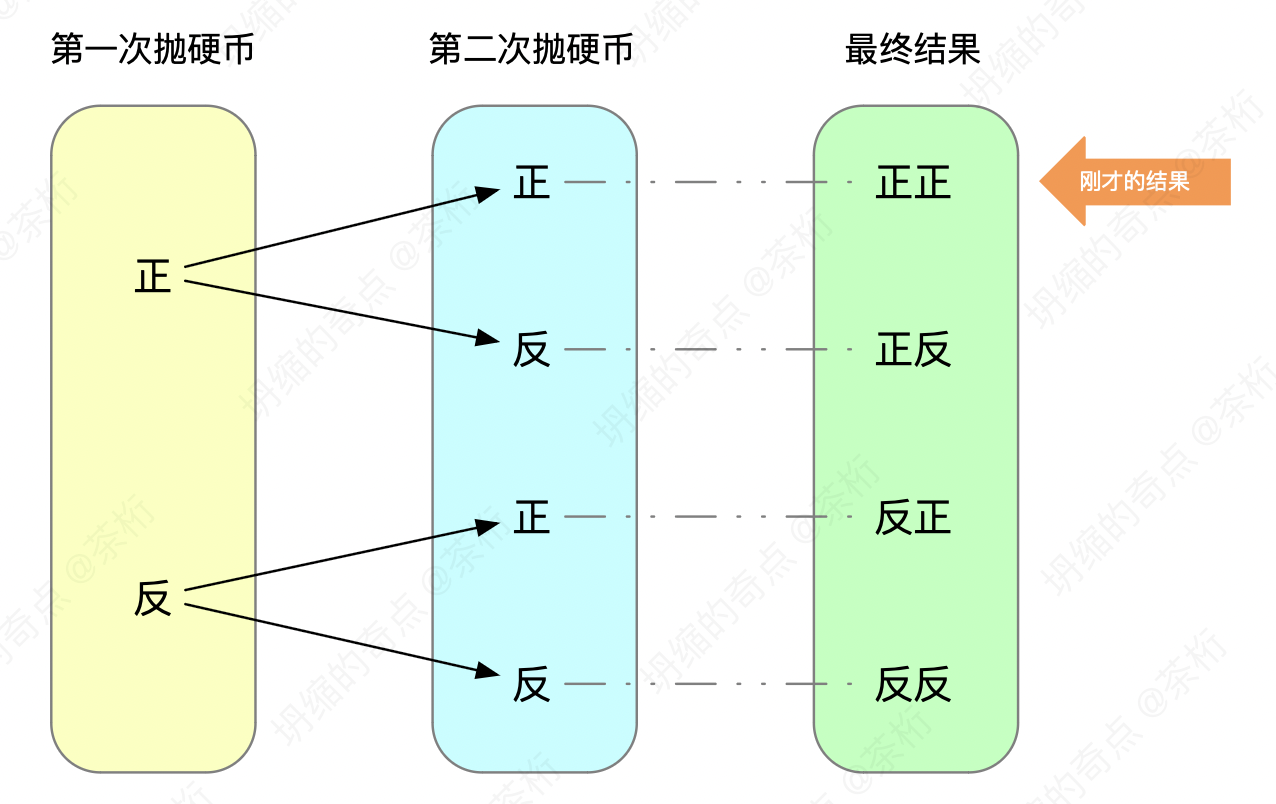
\includegraphics[width=0.7\textwidth]{asset/bd947955-687e-49b7-a430-c6921cd49504.png}
  \caption{抛硬币步骤}
  \label{fig:img5_2}
\end{figure}

首先来看一下, 第一次抛掷会出现两种结果, 要么正要么反. 第二次抛掷它是不是也有两种情况, 要么正要么反. 而第一次和第二次出现结果的组合总共有多少种? 是不是$2 \times 2 = 4$种? 就像这里的\textit{正正、正反、反正、反反}一共4种. 然后两次抛掷均为正面的情况, 只占一种, 所以它最终概率就是1/4. 总共有四种情况, 两次均为正只占一种情况, 所以不就是1/4吗? 

通过这个简单的例子得出一个什么样的结论呢? 就是这个事件如果由多个步骤完成的话最终可能出现的结果种类就是你每一步能出现的那个结果的数量相乘得到的. 

比如说第一步只可能出现正反两种结果, 第二步也是只可能出现要么正要么反两种结果, 那就是$2\times 2$总共等于4种结果. 如果再来第三次抛掷那又是多少, 就又是正或者反. 那就是$2\times 2\times 2=8$. 所以就引出了「联合概率」的这个概念. 

把A事件(就是第一次抛至正面朝上)发生的概率用$P(A)$表示. 

B事件(指第二次抛至正面朝上发生的概率)用$P(B)$来表示. 

A和B同时发生的概率用$P(AB)$或者$P(A,B)$来表示. 这两种都行, 都是等价的, 表示他们俩同时发生. 

如果A和B是相互独立的. 什么叫相互独立? 就是A发生不发生, 跟B一点关系都没有. 同样的B发生不发生, 跟A也没啥关系, 对A也没有任何影响, 你爱咋咋. 就像两口子吵架的一样, 你想干啥干啥, 你想剁手就剁手, 你想买东西买东西. 就是一个相互独立事件, 谁也不理谁谁也不需要管谁. 在这种情况下, 它们的联合概率就是它俩同时发生的概率, 也就是他们各自发生的概率乘在一起. 也就是说: \textbf{如果A和B它是相互独立的,则$P(AB) = P(A)P(B)$}

如果A和B它不是相互独立的, 那这个$P(AB)$它要怎么去计算呢? 这里就需要去通过一些概率的定义方面去做. 

\section{条件概率}

再来看一下第二个问题: 普通人和赌神抛硬币出现正面朝上概率是不一样的. 普通人正面朝上概率是0.5, 赌神正面朝上概率是0.7. 这两种概率表示同一种结果, 都是抛硬币正面朝上, 但是他们这个概率值是不一样的. 

\begin{itemize}
  \item 普通人 => P(正面朝上) = 0.5 
  \item 赌神 => P(正面朝上) = 0.7
\end{itemize}

单纯看这个P(正面朝上)我也判断不出来它这个概率究竟应该是0.5还是0.7. 所以在这里应该怎么样去处理呢? 虽然他俩都表示同样一种结果, 但是先决条件不一样, 一个是让普通人来抛, 另一个是让赌神来抛. 两个先决条件不一样, 最终结果肯定是不一样的. 所以在这里就引入了「\textbf{条件概率}」. 

\textbf{条件概率表示在某个先决条件已发生的情况下, 某一个事件发生的概率}. 先决条件与讨论的事件是有关联的, 就不像刚才那个例子里面说的一样, 第一次抛掷和第二次抛掷它是相互独立的, 谁也不用管谁, 在这里条件概率是有关联的. 

key $\Rightarrow$ 事件的先决条件不同

A在这里作为先决条件, 这个例子里面的先决条件就是操作者是赌神还是普通人. B是要讨论的研究的这个事件. 所以当A确定的情况下, B发生的概率用这个 $P(B|A)$ 来表示. 杠后面的条件已经发生的条件下, 杠前面的事件发生的概率有多少. 

在这里理解起来就是选定了普通人来抛硬币, 正面朝上的概率就是0.5, 正面朝上后面要加上一个杠, 然后在杠后面添加上普通人三个字:$P(B|\mbox{普通人})$

赌神也是一样, 在正面朝上后面添加上一个杠, 杠后面再加上赌神两个字: $P(B|\mbox{赌神})$.  表示操作者不同, 发生同一事件的概率是不一样的, 这个叫做条件概率. 

那联合概率和条件概率有什么联系吗? 

他们确实是有一些联系, 先来回顾一下联合概率: A和B是相互独立的, 那就等于它们各自发生的概率直接相乘得到的: $P(AB) = P(A)P(B)$

那如果A和B不是相互独立的怎么去计算它? 怎么计算A和B都发生的联合概率? 在这里就可以结合条件概率去做. 先求得A发生的概率是多少, 然后再来看A已经确定发生的情况下我B发生的概率是多少. 现在回过头来看刚才那个情景:\textbf{从赌神和普通人中随机选择一个人抛硬币}. 

$P(A)$代表从赌神和普通人两个人当中选出赌神的概率等于0.5对吧? 然后赌神抛出正面朝上的概率是0.7.  也就是在已经确定 A=赌神 的情况下, $P(B|A)$就相当于$P(B|\mbox{赌神})$, 抛出正面朝上的概率就等于0.7. 现在再来看$P(AB)$, 就等于$P(B|A)P(A)$, 所以就等于$0.5 \times 0.7=0.35$. 

总结一下联合概率:
\begin{itemize}
  \item 若A和B是相互独立的, 则 $P(AB) = P(A)P(B)$ 
  \item 若A和B不是相互独立的, 如何计算 $P(AB)$? 
  \item $key: P(AB) = P(B|A)P(A)$
\end{itemize}

这个部分其实还是已经很偏基础了, 正常逻辑思维能力都可以跟得上. 如果一时没跟上的也没有关系, 可能注意力不集中,再多看几遍就可以了, 自己再查查资料. 记住, \textbf{任何时候除了在课堂上学过的东西之外还需要拥有自学的能力}. 不管是在大学读本科、读研还是读博, 甚至说已经工作了, 或者说是在大学当老师怎么样, 如果没有自学的能力我觉得是很可怕的一件事情. 因为不可能所有的事情都能恰好找到适合你的那个老师或者机构帮你解决这个问题, 学习这个事还是要靠自己. 

再来看一下第三个问题: 第三个问题是前两次都是正面朝上, 那第三次抛掷还出现正面朝上的概率仍然是1/2吗? 答案是: 仍然是. 因为第几次, 就算是第n次也好, 它相互之间都无关. 第三次和第七次之间、和第六次、第五次、第十八次之间都是没有任何关联的, 都是独立的, 不相关. 所以第三次抛掷概率还是1/2. 

但是这一点有些人会觉得有点不大能理解为什么. 比如说, 在现实生活当中, 如果我连续抛四次硬币, 前三次都已经是正面了, 那第四次还是正面的概率就会觉得好像有点小. 但其实第四次出现正面朝上的概率仍然是1/2. 但是为什么会有这样的感觉, 就感觉好像第四次不大可能是正面了? 是因为心里面所想象出来这个概率小是针对什么事情来说, 概率小是\textbf{四次都出现正面朝上}这件事情概率小, 而不是\textbf{第四次抛出正面朝上}概率小, 这两个是不一样的. 

判断这两个事件是否独立的一个判断标准其实就是要看$P(B|A)$和$P(B)$它是否是相等. 如果他们俩是相等的就代表B发生的概率等于在A已经确定发生的情况下B发生的概率. 什么意思呢? 就是不管你A发生不发生, B的概率就是这么多, 那就是说A和B没有关系. A发生B的概率是这么多, A不发生B概率也是这么多, 这就是判断两个事件是否独立的一个标准. 

\section{随机事件}

接下来再来正式的说一下随机事件, 它表示在随机试验中可能出现也可能不出现, 而在大量重复试验中具有某种规律性的事件, 简称事件. 就比如下面这些例子:

\begin{itemize}
  \item 抛硬币, 正面朝上是一个随机事件
  \item 反面朝上亦是一个随机事件
  \item 掷骰子朝上的点数为偶数是一个随机事件. 
\end{itemize}

随机变量是什么概念? 刚才说随机事件, 因为想用数学化的语言去解决它, 去对它做一些处理. 所以希望能把这个随机事件的结果给它数量化表示, 数量化表示出来的这个结果就叫做随机变量. 

\begin{itemize}
  \item 一次随机试验可能出现的结果的数量化表示
  \item 一般用大写字母表示,  如X, Y
\end{itemize}

比如说我抛掷两个骰子得到的向上点数之和就是一个随机变量. 描述点数有可能用一个二元数组, 比如说第一个骰子4, 第二个骰子是2, 那在这种情况下可能就是用一对数来表示. 但是在这里, 通过点数之和可以把它转换成可操作的一个数量. 

\begin{itemize}
  \item 抛掷两个骰子得到的向上的点数之和就是一个随机变量
\end{itemize}

随机变量也分两种:「连续型」和「离散型」. 
\begin{itemize}
  \item 连续型随机变量, 如街头采坊一个人, 他/她的身高
  \item 离散型随机变量, 如街头采坊一个人, 他/她的性别
\end{itemize}

连续型就是随机变量的取值可以是连续的, 比如我街上在采访一个人, 他这个身高是178.65公分, 或者说他是164公分, 或者是183公分. 这个数值之间还有其他数值可以连续, 数字之间没有这种间隔, 不是跳跃性的. 更确切的说法解释就是: 178公分 - 180公分, 这两个确切数值之间还有其他的连续数值. 

离散型的随机变量就是有跳跃性的, 只能取规定的那些, 值与值之间是没有其他的值可以连续. 比如说在班上抽查学生, 抽出来是男生还是女生, 性别没办法用数字去表示, 所以就做一个转换, 比如说男生是-1女生是1, 那这样子就可以用随机变量的概念去处理这个概率事件. 男生对应着-1, 女生对应着+1, -1和+1之间没有其他值. 

做一些机器学习方面分类的时候其实也是一样的, 离散型的随机变量就是取值和取值之间没有相邻的量, 经常会把一些标记这种类别的东西给它转换为数字. 比如鉴别花的种类, 花可能有十几种, 如果按照中文名去做分类的话那计算机没办法对这种名字去做处理, 而在机器学习当中如果要鉴别花的种类, 把它转换成数字的形式去处理. 比如:月季对应着1, 玫瑰对应2, 百合对应5等等. 给它标一个数字, 实际上在机器学习的工程当中, 都是用独特编码还有其他的一些编码去做, 不是单纯的给它附一些值. 

\section{数学期望}

随机试验的结果可以有怎样定量的期待, 这个就表示了这个数学期望的一个含义. 什么意思呢? 就是有的时候, 在我做随机实验之前就能有一个大概的了解, 有一个预估. 如果做了这个实验我的回报, 或者说我的损失, 或者说这个实验结果会是怎么样的. 

比如一个人打算去赌博, 手里趁两钱去澳门了. 他有两种可能的结果, 一个是他赌赢了, 给他1,000美金, 概率只有0.001; 另一个就是他的赌资50美金打了水漂, 概率是0.999. 基本上就是赌赢的概率非常小. 赢都是小概率事件, 所以对于这两种结果他是可以提前预判到的. 那如何根据这些已经得到的信息来做一个对结果的预估呢? 这个就是数学期望. 就是能够获得的这个平均回报是多少, 就是说每种可能的结果(图: \ref{fig:img5_3}). 

\begin{figure}[ht]
  \centering
  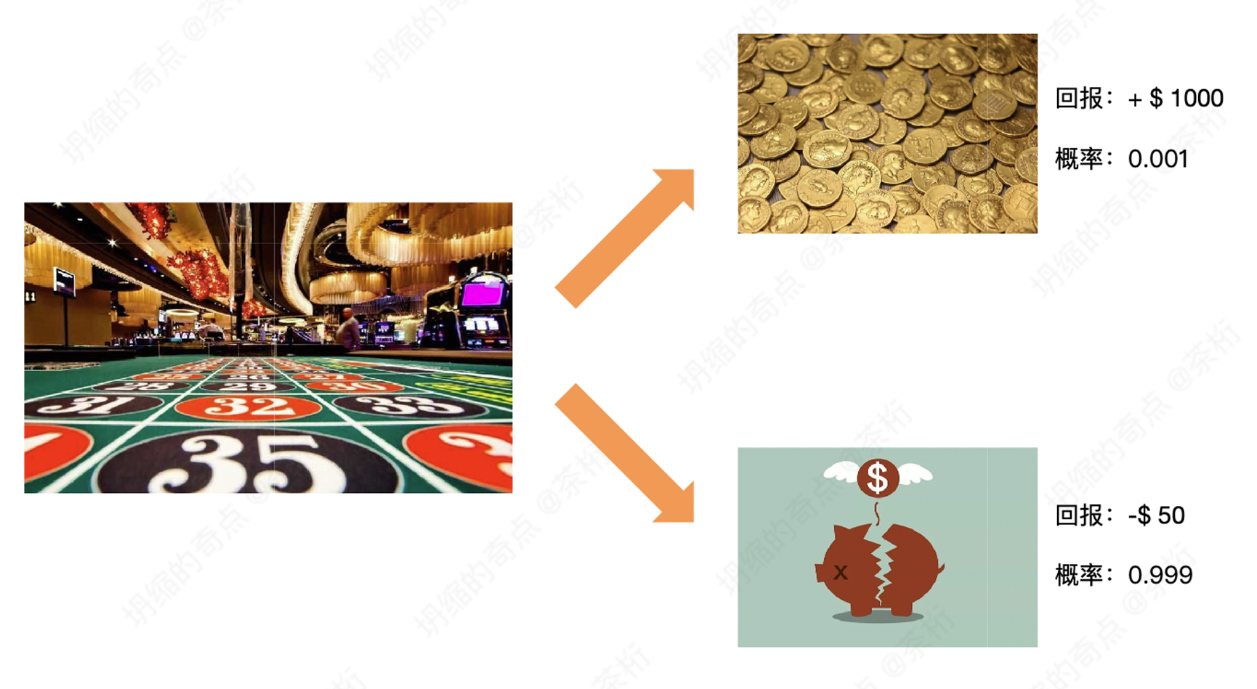
\includegraphics[width=1\textwidth]{asset/86da64b2-45f2-42c2-add4-d7db67f5cf82.png}
  \caption{}
  \label{fig:img5_3}
\end{figure}

在经过大量试验之后, 能够收到的平均回报是多少呢? 就是回报金额乘以概率, 最后两个计算结果相加:

\begin{align*}
  E(X) = 1000 \times 0.001 + (-50) \times 0.999 = -48.95
\end{align*}

这个$E(X)$就代表了数学期望, $E$ 代表了$\mathord{Expectation}$, 代表了期望. 这里的规则就是每种可能的结果乘上结果对应的概率, 再把所有的乘积加在一起, 其实也很简单对吧. 我相信大部分人听到这里都已经听懂了. 

那再来看下一个例子, 这个例子也很有趣: 有甲乙两个人进行赌博, 对于每一局而言,两个人获胜的几率都是相等的, 就是五五开, 谁也不占谁便宜. 比赛是五局三胜制, 最终的赢家可以获得100美元的奖励. 在第四局比赛开始前, 由于特殊情况需要终止比赛, 而在前三局甲已经赢了两局, 乙赢了一局. 那问题来了, 在没办法继续比赛的情况下, 应该如何公平的分配这100美元呢? 

就是说, 不把这后面两局给比出来的话不知道最终的结果, 因为前三局并不是甲都赢了或者乙都赢了, 甲只赢了两局乙只赢了一局, 谁都没有构成3胜. 所以这个时候就需要用到数学期望的知识去去判断一下, 甲如果这个比赛继续进行下去最终获胜的概率是多大, 然后通过他的这个获胜概率来预估一下他应该对应的奖金. 同样的对乙也做这样的判断, 如果比赛进行下去, 乙最终获胜的概率有多大. 然后根据获胜的概率来看一下乙他应该获得奖金的期望值是多少, 就是预估值是多少.

解: 若比赛继续, 甲只需要再赢一局即可获胜, 乙需要两场全赢. 

\begin{itemize}
  \item \textbf{甲}最终\textbf{不获胜}的概率: $P(\mbox{甲负}) = \frac{1}{2} \times \frac{1}{2} = \frac{1}{4} $
  \item \textbf{甲}最终\textbf{获胜}的概率: $P(\mbox{甲胜}) = 1 - P(\mbox{甲负}) = \frac{3}{4}$ 
  \item \textbf{乙}最终\textbf{获胜}的概率: $P(\mbox{乙胜})  = \frac{1}{2} \times \frac{1}{2} = \frac{1}{4}$ 
  \item \textbf{乙}最终\textbf{不获胜}的概率: $P(\mbox{乙负}) = 1 - P(\mbox{乙胜})  = \frac{3}{4}$ 
  \item 甲可获得的奖金期望值: $E(\mbox{甲}) = 100 \times \frac{3}{4} + 0 \times \frac{1}{4} = 75$ 
  \item 乙可获得的奖金期望值: $E(\mbox{乙}) = 100 \times \frac{1}{4} + 0 \times \frac{3}{4} = 25$
\end{itemize}

来一步一步看, 这个比赛如果比赛继续的话甲只需要再赢一局就可以了, 乙需要两场都赢. 所以最终甲他不获胜的概率, 假如说点背最后两局都输了, 那输的概率是$\frac{1}{2} \times \frac{1}{2}$, 乘在一起呢是1/4. 这就是甲最终不获胜的概率. 

然后就知道了, 甲最终要么获胜要么不获胜, 只有这两种结果, 不可能出现第三种情况. 就拿1去减这种情况, 就对应的这个甲最终获胜的概率. 甲获胜的所有情况加在一起概率之和为1, 通过1去减1/4就得到3/4. 

同样的道理, 乙也是一样, 乙必须两场全赢, 所以乘在一起等于1/4. 乙最终不获胜也拿1去减, 等于3/4. 

再来分别看一下, 按照数学期望的定义, 甲如果继续比赛下去有哪两种结果? 赢或者不赢. 赢对应的奖金有100, 概率呢是3/4, 输的奖金就是零, 一分钱没有, 甲输的概率是1/4, 所以甲获得奖金的期望值是75. 

乙去做同样的运算, 获胜的概率是1/4, 获胜了也是能拿100块钱, 再加上不获胜就一分钱没有, 不获胜概率3/4. 这么一乘一加, 乙获得奖金的期望值就是25. 

所以按照75和25的分配方式把奖金给甲和乙分了就行了, 而且保证公平公正, 因为是根据两人各自的胜率、期望值来得到的, 所以是公平的. 

期望还有一些性质:

\begin{enumerate}
  \item $E(C) = C$, $C$ 为常数 
  \item $E(CX) = CE(X)$, $C$ 为常数 
  \item $E(X+Y) = E(X) + E(Y)$ 
  \item $E(XY) = E(X)E(Y)$,  当$X,Y$相互独立时
\end{enumerate}

第一个, 如果是对一个常数去求期望的话, 就是参数本身. 就像常函数一样, $f(x) = 3$, 始终都是3. 

第二个性质, $E$乘上$CX$, 就是它的随机变量乘上一个常数, 等于把这个常数拿出来和这个随机变量的期望值相乘. 

如果是两个随机变量相加, 是把他们各自的期望值加在一起, 等于他们俩相加的期望值. 

如果两个随机变量相乘只有当X和Y相互独立的时候这个式子才成立. $E(XY)$等于$E(X)$乘上$E(Y)$. 如果X、Y不是相互独立的话, 就只能根据这个期望值的定义去做. 期望值的定义就是每种结果乘上这个结果对应的概率值, 再把所有的乘积加在一起. 

\section{方差}

思考一个例子: 投掷一枚骰子, 它向上的点数期望值是多少呢? 来计算一下:

\begin{align*}
  E(\mbox{点数}) & = \frac{1}{6} \times 1 + \frac{1}{6} \times 2 + \frac{1}{6} \times 3 + \frac{1}{6} \times 4 + \frac{1}{6} \times 5 + \frac{1}{6} \times 6 \\
  & = 3.5
\end{align*}

根据这个计算,$1 \quad 2 \quad 3 \quad 4 \quad 5 \quad 6$ 出现机会均等, 都是1/6, 算出来结果期望值点数3.5. 但是朝上点数不可能总是3或者4, 各个点数出现的次数都是均等的. 所以单纯的靠期望值这么一个量去表示一个随机事件可能会有其他一些方面信息的缺失. 也就是说这句话里面出现的矛盾, 期望值3.5似乎是在3和4之间出现的情况最多, 但是实则是各个点数都一样, 怎么刻画呢? 

这里就用到了方差的概念. 方差是度量随机变量和它的数学期望之间偏离程度的一个量. 定义式: 

\begin{align*}
  D = \sigma ^2 = \sum^N_{i=1} \frac{(X-E(X))^2}{N}
\end{align*}

定义式中, 一般用大写字母D来表示, 也可以用$\sigma^2$来表示. 如果给它开个平方的话, 就叫做标准差. 之后也会说到标准差, 标准差用一个$\sigma$来表示. 

等号后面就是这里面所有种情况($\sum_{i=1}^N$), 每种情况的取值($X$)减去数学期望的值($E(X)$), 再做一个平方, 然后再除以每一个情况可能出现的这个概率(N). 在这里机会均等, 就像投骰子一样, $1 \quad 2 \quad 3 \quad 4 \quad 5 \quad 6$ 点数朝上概率是均等的. 所以除以一个N, 这个就是方差的一个定义. 

那方差可以帮助去做什么呢? 在这里看一个例子:

A和B两个人工智能模型, 它们在一系列同分布的数据集上的分类准确率如表\ref{fig:table5_1}所示, 判断哪个模型表现更好:

\begin{table}[ht]
  \centering
  \begin{tabular}{lllllll}
  \midrule
    A & 90\% & 92\% & 93\% & 91\% & 92\% & 94\%\\
    B & 88\% & 97\% & 90\% & 96\% & 94\% & 87\%\\
  \bottomrule
  \end{tabular}
  \caption{A和B的分类准确率}
  \label{fig:table5_1}
\end{table}

现在有A和B两个人工智能模型, 它们在一系列同分布的数据集上的分类准确率就如上面展示的这样. 现在需要判断哪一个模型表现更好. 

同分布的意思就是它们俩判断的数据集概率模型是一样的, 不可能出现一个是高斯分布, 一个是泊松分布. 这两个本来分布都不一样的模型, 判断精确度就不可能去做一个评判了, 所以肯定是同分布, 或者说就是同样的数据集, 同样的数据集去做这个分类. 

总共判别6次, A的准确率是第一行表示, B的准确率是第二行表示. 

先从均值, 也就是数学期望的角度去判断一下, 看他们有没有优劣之分. 

\begin{align*}
  E(A) = \frac{90\% + 92\% + 93\% + 91\% + 92\% + 94\%}{6} = 92\% \\
  E(B) = \frac{88\% + 97\% + 90\% + 96\% + 94\% + 87\%}{6} = 92\%
\end{align*}

A通过运算得出来结果是92\%, 各次分类的结果平均而言准确率是92\%. 就是说92\%的样本A模型可以正确识别, 剩下8\%判断错误. 

B运算得到的也是92\%. 所以从均值或者说期望的角度去判断是没办法说哪个好哪个不好. 

这时候再来看一下方差, 从方差的角度判断 \textit{(由于公式过长会导致板式出错,所以将原本一行的相加折成了两行)}:

\begin{align*}
  \sigma^2(A) & = \frac{(0.9-0.92)^2 + (0.92-0.92)^2 + (0.93-0.92)^2}{6} \\ & + \frac{(0.91-0.92)^2 + (0.92-0.92)^2 + (0.94-0.92)^2}{6} \\ 
  & = 0.000167 \\
  \sigma^2(B) & = \frac{(0.88-0.92)^2 + (0.97-0.92)^2 + (0.90-0.92)^2}{6} \\ & + \frac{(0.96-0.92)^2 + (0.94-0.92)^2 + (0.88-0.92)^2}{6} \\
  & = 0.00135 \\ 
  \mbox{因为}: & \quad  \sigma^2(A) < \sigma^2(B) \\
  \mbox{所以}: & \quad \mbox{模型A的表现更稳定更好. }
\end{align*}

A的方差计算后数值为$0.000167$, B是$0.00135$ \footnote{这里是我自己手工计算得到结果和程序计算相印证, 应该是没有错误的. }. 

然后就判断出来A的方差比B的方差要小, 小代表什么呢? 回忆一下方差里面的定义, 就是这个随机变量离期望的偏离程度. 那方差越小就代表偏离程度越小, 偏离程度越小代表这个模型表现的比较稳定, 比较稳定就不会起伏很大. 

有些同学可能状态起伏特别大, 这次能考班上第一, 下一次有可能就只能考班上第十几名. 从这个角度来看A模型的表现就比B要更稳定, 所以模型A的表现更好. 这就是方差可以帮我们做的事情. 

有的同学可能要问: 为什么在方差的定义式里面要加上平方这项? 不用平方不行吗? 

Why平方? $\sigma^2 = \sum^N_{i=1}\frac{(X-E(X))^2}{N} \quad ?$.

不用平方不可以吗? $\sigma = \sum^N_{i=1}\frac{X-E(X)}{N} \quad ?$

确实是不行, 比如说图\ref{fig:img5_4} 的例子:

\begin{figure}[ht]
  \centering
  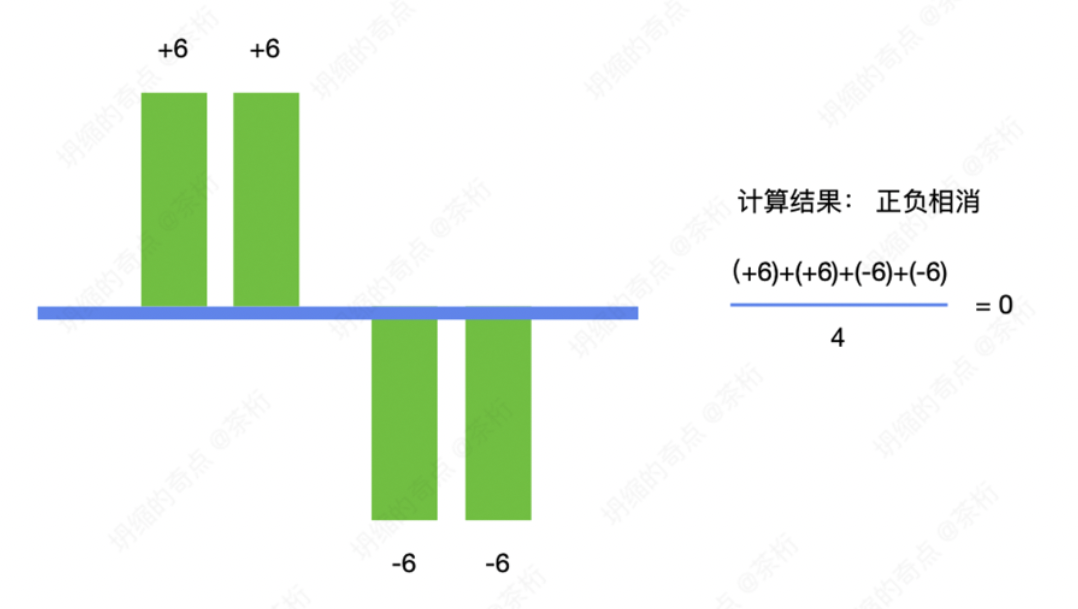
\includegraphics[width=0.9\textwidth]{asset/713e717f-8a86-42db-83e6-b74c5afe50a4.png}
  \caption{}
  \label{fig:img5_4}
\end{figure}

蓝色的横线代表均值, 也就是期望. 绿色的柱子代表了各个量, 相对于数学期望的一个偏差值. 比如结果比数学期望分别为(+6,  +6,  -6,  -6), 如果不把它平方一下, 会发现它就正负相消了, 最终得出的结论方差为零. 那这是显然不可能的事对吧? 所以要在这里加一个平方. 

有的脑子好一点的同学可能还会问: 那绝对值行不行? 绝对值按照道理来说其实是可以的, 没有问题. 但是绝对值运算在数学处理里面不太好去处理, 因为还得判断绝对值符号. 比较什么时候取正、什么时候取负, 这样子去做的话用平方会比较好一点. 

\hypertarget{方差的性质}{}
来看一下方差的一些性质:

\begin{enumerate}
  \item $D(C)=0$,  $C$ 为常数
  \item $D(X+C) = D(X)$, $C$ 为常数
  \item $D(CX) = C^2D(X)$, $C$ 为常数
  \item $D(X+Y) = D(X) + D(Y) + 2Cov(X,Y)$ \hyperlink{协方差}{$Cov$ 意为协方差}
  \item $D(X+Y) = D(X) +D(Y)$,  当X和Y相互独立时
  \item $Cov(X, Y) = E\{[X - E(X)][Y-E(Y)]\}$:  协方差
\end{enumerate}

方差的性质就是这些, 对于常数而言方差是0, 因为很显而易见, 它都没有偏离了, 始终取值就那一个, 就等于0. 

以上的这些式子, 大家看一下就好, 就不再一一缀述了. 

\section{标准差}

接下来就说说标准差, 标准差我刚才提到过, 直接对方差开个平方($\sqrt{D}$). 他有一个好处就是, 度量的效果和方差是一致的. 

\begin{align*}
  \sigma  = \sqrt{\sum^N_{i=1}\frac{(X-E(X))^2}{N}}
\end{align*}

设想一下, 一个量的方差大于另外一个量的方差, 比如说A大于B, 那开平方之后, 标准差还是保持一致的. 大小关系不会变. 但是标准差有一个好处, 方差因为有一个平方, 所以它和随机变量的\textit{量纲}是不一致的. 开一个平方之后, 在量纲方面就能和随机变量保持一致. 

量纲其实就是单位, 千克、米、秒这些叫做量纲, 其实就是单位. 所以标准差:

\begin{itemize}
  \item 度量效果与方差一致
  \item 量纲和随机变量一致
\end{itemize}

\hypertarget{协方差}{}
\section{协方差}

我们在上面\hyperlink{方差的性质}{方差的性质}中,其中引出了这么一个量, 第4个式子 $D(X+Y) = D(X) + D(Y) + 2Cov(X,Y)$: 当两个随机变量加在一起, 考虑他们和的方差的时候, 是等于各自的方差再加上一个 $2Cov(X,Y)$, 这个概念叫做协方差\textit{Covariance} . 

协方差是用于衡量两个变量的总体误差. 说通俗点就是, 当协方差是正的, 就代表这两个随机变量的变化趋势是相同的. 如果随机变量A大于期望值的时候, 随机变量B也应该大于他的期望值. 如果是小于的情况也是一样. 两个大于同时大于, 两个小于也同时小于. 

如果协方差为负, 那这两个变量的变化趋势就相反了. 一个大于期望值, 另外一个小于, 反过来也是成立的. 

协方差为0的时候代表两个变量没有线性相关性. 

这个「线性相关性」很多书本上面把「\textbf{线性}」两个字给去掉了, 只提「相关性」. 其实是不对的, 如果把\textbf{线性}给去掉, 只说两个变量无相关性, 无相关性就对应着两个变量独立, 但是两个变量除了线性的相关性之外, 还可以有其他非线性的. 

那什么叫线性呢? 也就是说$Y=K(X+B)$这种形式,当X变换的时候,Y也是按照这个放大倍数变换的. 

再换一个严格意义上的例子: $Y=KX$ 这个例子, X扩大K倍Y也是K倍的扩大多少, 这种叫做线性. 

而非线性呢, 比如说$Y=X^2$, X增加了多少, Y增加的量不是乘上一个常数来决定的, 这种叫做非线性. 

所以协方差为0只能说两个变量没有线性相关性, 不能得出两个变量是独立的. 

总结一下协方差:

\begin{itemize}
  \item 用于衡量两个变量的总体误差
  \item 协方差为正: 两个变量的变化趋势相同, 当一个大于其期望值时, 另一个也大于, 小于的情况亦然.
  \item 协方差为负: 两个变量的变化趋势相反, 当一个大于其期望值时, 另一个就小于, 反之亦然.
  \item 协方差为0: 两个变量无线性相关性.
  \item 两个变量独立, 则协方差一定为0, 反之并不一定成立.
\end{itemize}

所以, 协方差为0不一定得出来变量是独立的. 这个可能稍微有点绕, 但是大家只要能把\textit{线性相关性}、\textit{非线性相关性}和\textit{独立}给区别出来就行. 来看一下相关公式:

\begin{align*}
  Cov(X,Y) & = E\{[X-E(X)][Y-E(Y)]\} \\
  & = E\{XY - XE(Y) - YE(X) + E(X)E(Y)\} \\
  & = E(XY) - E[XE(Y)] - E[YE(X)] + E(X)E(Y) \\
  & = E(XY) - E(X)E(Y) - E(X)E(Y) + E(X)E(Y) \\
  & = E(XY) - E(X)E(Y)
\end{align*}

经过一系列运算得到两个随机变量的协方差, 可以表示成两个乘积的期望值减去期望值的乘积. 所以如果$X,Y$是独立的, 那E(XY)等于什么?

当$X, Y$独立时, $E(XY) - E(X)E(Y) = 0 \Rightarrow Cov(X,Y) = 0 $.

接下来这个内容其实就是体现了或者说验证了刚才说的. 就是两个随机变量的协方差如果是正的就代表增长的方向是相同的. 如果是负的就代表了一个增就一个减、一个减就一个增. 

例:表\ref{fig:table5_2} 给出一位同学的历次数学和物理考试的乘积, 试利用协方差判断他的两个科目成绩之间有怎样的关系. 

\begin{table}[ht]
  \centering
  \begin{tabular}{lllllll}
    \midrule
      数学 & 90 & 92 & 85 & 97 & 96 & 98 \\
      物理 & 85 & 95 & 88 & 95 & 93 & 90 \\
    \bottomrule
  \end{tabular}
  \caption{成绩单}
  \label{fig:table5_2}
\end{table}

\begin{align*}
  \mbox{解: \qquad E(数)} & = \frac{90+92+85+97+96+98}{6} = 93 \\ \\
  \mbox{E(物)} & = \frac{85+95+88+95+93+90}{6} = 91 \\ \\
  \mbox{E(数、物)} & = \frac{90 \times 85+92 \times 95 + 85 \times 88 + 97 \times 95 + 96 \times 93 + 98 \times 90}{6} \\ 
  & = 8472.17 \\ \\
  \mbox{两个变量的协方差:} \\  
  Cov(\mbox{数,物理}) & = E(\mbox{数,物}) - E(\mbox{数})E(\mbox{物理}) \\ 
  & = 8472.17 - 93 \times 91 = 9.17
\end{align*}

计算下来,运算得到结果是9.17, 它是大于零的, 所以代表这两个学科的成绩是成一个正相关的关系. 

再来思考一个问题: 大于0的时候, 协方差越大, 关联性越大嘛? 

对于同样的随机变量而言是这样没错. 就比如这一位同学的数学和物理考试成绩, 他又考了几次, 又有了新的数据, 计算出来结果可能比这个9.17大或者小, 那这个时候就可以拿9.17和新的计算出来的协方差的数值去进行一个比较, 越大这个相关性就越大. 

但是如果是不同的随机变量之间就没办法说了. 所以这里有一个概念叫做「相关系数」. 就是协方差除以随机变量的方差, 就把它做一个归一化的处理, 消除了数值本身带来的影响, 那这个就是「简单相关系数」. 还有其它一些不同的相关系数, 比如复相关系数、典型相关系数等等. 关于「相关系数」, 强烈建议大家下来再自己查询一下. 